\documentclass{article}
% generated by Madoko, version 1.0.0-rc5
%mdk-data-line={1}


\usepackage[heading-base={2},section-num={False},bib-label={True}]{madoko2}


\begin{document}



%mdk-data-line={7}
\mdxtitleblockstart{}
%mdk-data-line={7}
\mdxtitle{\mdline{7}Optimization of a DNN Program on the CPU+MIC Platform}%mdk
\mdxauthorstart{}
%mdk-data-line={12}
\mdxauthorname{\mdline{12}University of Electronic Secience and Technology of China}%mdk
\mdxauthorend\mdtitleauthorrunning{}{}\mdxtitleblockend%mdk

%mdk-data-line={9}
\begin{abstract}%mdk

%mdk-data-line={10}
\noindent\mdline{10}This article is a part of competition proposal of Asia Supercomputer Student Challenge. We analysis the \mdline{10}\mdcode{DNN}\mdline{10} program, put forward different optimization methods, test them and point their pros and cons. In the end we talk about our limitations.%mdk
%mdk
\end{abstract}%mdk

%mdk-data-line={12}
\section{\mdline{12}1.\hspace*{0.5em}\mdline{12}Introduction}\label{sec-introduction}%mdk%mdk

%mdk-data-line={13}
\noindent\mdline{13}There is a program based on a standalone hybrid CPU+MIC platform called \mdline{13}\mdcode{DNN(deep~neural~network)}\mdline{13} needed to be parallelized for obtain better performance. Here is some detailed information about hardware in Figure 1, software configuration in Figure 2.%mdk

%mdk-data-line={15}
\mdline{15}After optimization, the final program is tested on one computing server in the CPU+MIC hybrid cluster. Performance analysis in this proposal is based on the results of this test.%mdk

%mdk-data-line={16}
\begin{figure}[tbp]%mdk
\begin{mdcenter}%mdk

%mdk-data-line={18}
\noindent\mdline{18}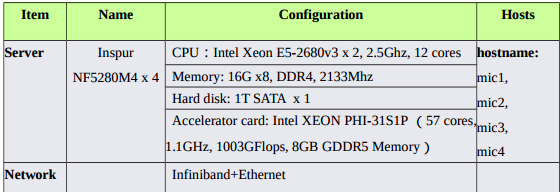
\includegraphics[keepaspectratio=true,width=\dimmin{}{\dimwidth{0.90}}]{images/2016-02-18-23-01-13-}{}\mdline{18}%mdk

%mdk-data-line={21}
\mdhr{}%mdk

%mdk-data-line={22}
\noindent\mdline{22}\mdcaption{\textbf{Figure~\mdcaptionlabel{1}.}~\mdcaptiontext{Hardware configuration}}%mdk
%mdk
\end{mdcenter}\label{fig-myfigure}%mdk
%mdk
\end{figure}%mdk

%mdk-data-line={23}
\begin{figure}[tbp]%mdk
\begin{mdcenter}%mdk

%mdk-data-line={24}
\noindent\mdline{24}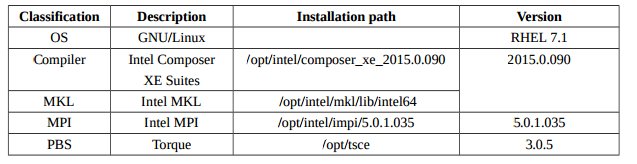
\includegraphics[keepaspectratio=true,width=\dimmin{}{\dimwidth{0.90}}]{images/2016-02-18-23-13-11-}{}\mdline{24}%mdk

%mdk-data-line={27}
\mdhr{}%mdk

%mdk-data-line={28}
\noindent\mdline{28}\mdcaption{\textbf{Figure~\mdcaptionlabel{2}.}~\mdcaptiontext{Software configuration}}%mdk
%mdk
\end{mdcenter}\label{fig-myfigure}%mdk
%mdk
\end{figure}%mdk

%mdk-data-line={29}
\section{\mdline{29}2.\hspace*{0.5em}\mdline{29}Analysis of the Serial Program}\label{sec-analysis-of-the-serial-program}%mdk%mdk

%mdk-data-line={30}
\subsection{\mdline{30}2.1.\hspace*{0.5em}\mdline{30}Coarse Grain Analysis}\label{sec-coarse-grain-analysis}%mdk%mdk

%mdk-data-line={31}
\noindent\mdline{31}At first, we generate a call graph(Figure 3) by using \mdline{31}\mdcode{Google~perfools}\mdline{31}, a open source performance profiler, to have a glance though it. Every square represents a function, and the bigger square is, the more time corresponding function cost.%mdk

%mdk-data-line={33}
\begin{figure}[tbp]%mdk
\begin{mdcenter}%mdk

%mdk-data-line={34}
\noindent\mdline{34}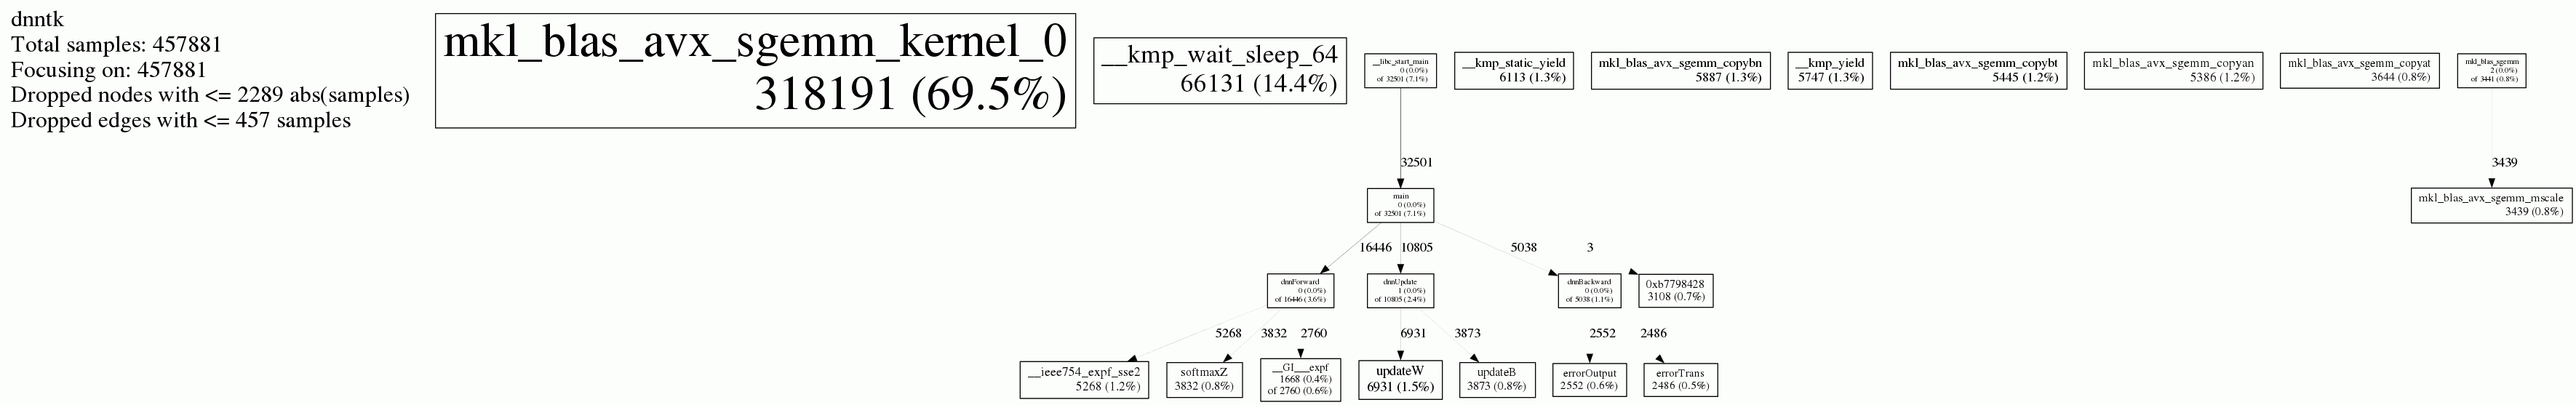
\includegraphics[keepaspectratio=true,width=\dimmin{}{\dimwidth{0.90}}]{images/100001994364201}{}\mdline{34}%mdk

%mdk-data-line={37}
\mdhr{}%mdk

%mdk-data-line={38}
\noindent\mdline{38}\mdcaption{\textbf{Figure~\mdcaptionlabel{3}.}~\mdcaptiontext{Google Perfools results}}%mdk
%mdk
\end{mdcenter}\label{fig-myfigure}%mdk
%mdk
\end{figure}%mdk

%mdk-data-line={38}
\mdline{38}Obviously, the hot spot is something about \mdline{38}\mdcode{MKL}\mdline{38}. After googling
and searching Intel document we know that MKL provides \mdline{39}\mdcode{BLAS~routinues}\mdline{39}, which includes a serial function named \mdline{39}\mdcode{cblas\_?gemm}\mdline{39}
to compute a matrix-matrix product with general matrices.%mdk

%mdk-data-line={42}
\mdline{42}But giving that MKL function is well-optimized, we search for all position where \mdline{42}\mdcode{cblas\_*gemm}\mdline{42} is called. Results show the usage of \mdline{42}\mdcode{cblas\_*gemm}\mdline{42} appear in file \mdline{42}\mdcode{dnn\_func.cpp}\mdline{42}, more specifically, in three functions:%mdk

%mdk-data-line={44}
\begin{itemize}[noitemsep,topsep=\mdcompacttopsep]%mdk

%mdk-data-line={44}
\item\mdline{44}\mdcode{\preindent{1}extern~"C"~int~dnnForward(NodeArg~\&nodeArg)}\mdline{44}%mdk

%mdk-data-line={45}
\item\mdline{45}\mdcode{\preindent{1}extern~"C"~int~dnnBackward(NodeArg~\&nodeArg)}\mdline{45}%mdk

%mdk-data-line={46}
\item\mdline{46}\mdcode{\preindent{1}extern~"C"~int~dnnUpdate(NodeArg~\&nodeArg)}\mdline{46}

%mdk-data-line={47}
\begin{figure}[tbp]%mdk
\begin{mdcenter}%mdk

%mdk-data-line={48}
\noindent\mdline{48}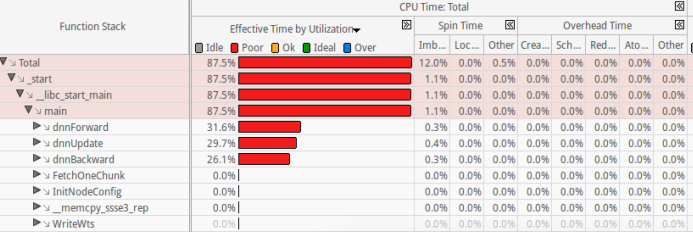
\includegraphics[keepaspectratio=true,width=\dimmin{}{\dimwidth{0.90}}]{images/2016-02-19-10-36-25-}{}\mdline{48}%mdk

%mdk-data-line={50}
\mdhr{}%mdk

%mdk-data-line={51}
\noindent\mdline{51}\mdcaption{\textbf{Figure~\mdcaptionlabel{4}.}~\mdcaptiontext{Intel VTune top-down tree}}%mdk
%mdk
\end{mdcenter}\label{fig-myfigure}%mdk
%mdk
\end{figure}%mdk%mdk
%mdk
\end{itemize}%mdk

%mdk-data-line={52}
\noindent\mdline{52}They call \mdline{52}\mdcode{MKL}\mdline{52} function \mdline{52}\mdcode{cblas\_sgemm}\mdline{52} many times by \mdline{52}\mdcode{for~loop}\mdline{52} and 
cost almost 90\% of all CPU time. So we guess that those function
 is what we may optimize, aka, hotspots.
The report(see Figure 4.) showed by\mdline{55}\mdcode{Intel~VTune}\mdline{55}, another profiler, proves our guess.%mdk

%mdk-data-line={59}
\mdline{59}According to a skim through the source code, we could establish a clear structure about this program. To simplify code, original program could be rewritten in pseudocode:%mdk
\begin{mdpre}%mdk
\noindent{\mdcolor{purple}1}.~{\mdcolor{teal}GetInitFileConfig}(cpuArg)\\
{\mdcolor{purple}2}.~{\mdcolor{teal}While}~{\mdcolor{teal}FetchOneChunk}(cpuArg,~onChunk)~{\mdcolor{navy}do}:\\
{\mdcolor{purple}3}.~~~~~~~{\mdcolor{teal}While}~{\mdcolor{teal}FetchOneBunch}(oneChunk,~nodeArg)~{\mdcolor{navy}do}:\\
{\mdcolor{purple}4}.~~~~~~~~~~~~dnnForward(nodeArg)\\
{\mdcolor{purple}5}.~~~~~~~~~~~~dnnBackward(nodeArg)\\
{\mdcolor{purple}6}.~~~~~~~~~~~~dnnUpate(nodeArg)\\
{\mdcolor{purple}7}.~{\mdcolor{teal}WriteWts}(nodeArg,~cpuArg)\\
{\mdcolor{purple}8}.~{\mdcolor{teal}UninitProgramConfig}(cpuArg)\\
%mdk
\end{mdpre}\noindent\mdline{71}There are two nested loop before \mdline{71}\mdcode{dnn*()}\mdline{71} series, and 
in each of those processing function many matrix-matrix product are
executed. Whether those hotspots could be parallelized or not depends
on data scale, dependency and so on. Before we discuss some methods and weighed their pros and cons the implementation of \mdline{74}\mdcode{DNN}\mdline{74} should be most carefully checked.

%mdk-data-line={76}
\subsection{\mdline{76}2.2.\hspace*{0.5em}\mdline{76}Fine Grain Analysis}\label{sec-fine-grain-analysis}%mdk%mdk

%mdk-data-line={78}
\subsubsection{\mdline{78}2.2.1.\hspace*{0.5em}\mdline{78}Matrix Size}\label{sec-matrix-size}%mdk%mdk

%mdk-data-line={80}
\noindent\mdline{80}All \mdline{80}\mdcode{cblas\_sgemm}\mdline{80} is called like this:%mdk
\begin{mdpre}%mdk
\noindent~~cblas\_sgemm({\mdcolor{teal}CblasRowMajor},~{\mdcolor{teal}CblasNoTrans},~{\mdcolor{teal}CblasNoTrans},\textbackslash{}\\
~~~~~~~~numN,~numA[i],~numA[i-{\mdcolor{purple}1}],~\textbackslash{}\\
~~~~~~~~one,~d\_Y[i-{\mdcolor{purple}1}],~numA[i-{\mdcolor{purple}1}],~d\_W[i],~numA[i],\\
~~~~~~~~one,~d\_Y[i],~numA[i]);%mdk
\end{mdpre}\noindent\mdline{87}The arguments \mdline{87}\mdcode{numN}\mdline{87}, \mdline{87}\mdcode{numA[i]}\mdline{87}, \mdline{87}\mdcode{numA[i-1]}\mdline{87} indicating the size of the matrices:

%mdk-data-line={89}
\begin{itemize}[noitemsep,topsep=\mdcompacttopsep]%mdk

%mdk-data-line={89}
\item\mdline{89}\mdcode{d\_Y[i-1]}\mdline{89} is a \mdline{89}\mdcode{numN}\mdline{89} row by \mdline{89}\mdcode{numA[i]}\mdline{89} column matrix;%mdk

%mdk-data-line={90}
\item\mdline{90}\mdcode{d\_W[i]}\mdline{90} is a \mdline{90}\mdcode{numN}\mdline{90} row by \mdline{90}\mdcode{numA[i-1]}\mdline{90} column matrix;%mdk

%mdk-data-line={91}
\item\mdline{91}\mdcode{d\_Y[i]}\mdline{91} is a \mdline{91}\mdcode{numA[i-1]}\mdline{91} row by \mdline{91}\mdcode{numA[i]}\mdline{91} column matrix.%mdk
%mdk
\end{itemize}%mdk

%mdk-data-line={93}
\noindent\mdline{93}As we known the bigger matrix size is, the higher degree of \mdline{93}\mdcode{MKL}\mdline{93} parallelism is. But in the \mdline{93}\mdcode{DNN}\mdline{93} program, the size of matrix is decided by \mdline{93}\mdcode{bunchSize}\mdline{93}, a constant integer (\mdline{93}\ensuremath{\approx}\mdline{93}1024), and element (\mdline{93}\ensuremath{\approx}\mdline{93}1024) of \mdline{93}\mdcode{dnnLayerArr}\mdline{93}, a constant integer array. The two integers are configured by specified file, and we are not allowed to modify it. For this reason there are no sufficiently large matrix to enable \mdline{93}\mdcode{auto~offload~model}\mdline{93} to speed up \mdline{93}\mdcode{DNN}\mdline{93}.\mdline{93}[\mdcite{mkl-mic}{2}]\mdline{93}%mdk

%mdk-data-line={95}
\subsubsection{\mdline{95}2.2.2.\hspace*{0.5em}\mdline{95}Cycles Index}\label{sec-cycles-index}%mdk%mdk

%mdk-data-line={96}
\noindent\mdline{96}In the \mdline{96}\mdcode{dnn*}\mdline{96} series every loop call \mdline{96}\mdcode{cblas\_sgemm}\mdline{96} \mdline{96}\mdcode{numN}\mdline{96}(\mdline{96}\ensuremath{\approx}\mdline{96}7) times, which indicates the length of \mdline{96}\mdcode{dnnLayerArr}\mdline{96}. It\mdline{96}'\mdline{96}s regretful that the value cannot be modified by us. Giving the number of core(\mdline{96}\ensuremath{\approx}\mdline{96}24 in CPU or \mdline{96}\ensuremath{\approx}\mdline{96}60 in MIC) and constant \mdline{96}\mdcode{numN}\mdline{96}, it\mdline{96}'\mdline{96}s not wise to parallelize those loops.%mdk

%mdk-data-line={98}
\section{\mdline{98}3.\hspace*{0.5em}\mdline{98}Parallelization Design Methods}\label{sec-parallelization-design-methods}%mdk%mdk

%mdk-data-line={100}
\subsection{\mdline{100}3.1.\hspace*{0.5em}\mdline{100}Fine Grain Parallelism}\label{sec-fine-grain-parallelism}%mdk%mdk

%mdk-data-line={102}
\noindent\mdline{102}In function \mdline{102}\mdcode{dnnForward}\mdline{102}, it\mdline{102}'\mdline{102}s easy to observe there is a loop invoking \mdline{102}\mdcode{cblas\_sgemm}\mdline{102}, which nearly cost all CPU time consumed by this function. So it\mdline{102}'\mdline{102}s same with the \mdline{102}\mdcode{dnnBackward}\mdline{102} and \mdline{102}\mdcode{dnnUpdate}\mdline{102}. A rough thoughts occurred to us that we could parallelize this \mdline{102}\mdcode{for~loop}\mdline{102} using multi-threads. But data dependency in \mdline{102}\mdcode{for~loop}\mdline{102} and relatively small cycle index make it inefficient to parallelize. So   we should consider generalizing the parallelization region to smaller scale. Taking the feature of \mdline{102}\mdcode{MIC}\mdline{102} in to account we hope to execute highly parallel code and/or compute intensive code in the \mdline{102}\mdcode{MIC}\mdline{102}. Focusing on \mdline{102}\mdcode{dnn*}\mdline{102} series it\mdline{102}'\mdline{102}s easy to find an abstract structure to generalize them:%mdk
\begin{mdpre}%mdk
\noindent~~extern~{\mdcolor{maroon}"}{\mdcolor{maroon}C}{\mdcolor{maroon}"}~{\mdcolor{navy}int}~dnn***({\mdcolor{teal}NodeArg}~\&nodeArg)\\
\{\\
~~~~{\mdcolor{darkgreen}/*}{\mdcolor{darkgreen}~Variables~definition~}{\mdcolor{darkgreen}*/}\\
~~~~{\mdcolor{navy}float}~~*d\_X~=~nodeArg.d\_X;\\
~~~~~~...\\
~~~~{\mdcolor{darkgreen}/*}{\mdcolor{darkgreen}~Preprcess~function~func1~}{\mdcolor{darkgreen}*/}\\
~~~~func1(...);\\
\\
~~~{\mdcolor{darkgreen}/*}{\mdcolor{darkgreen}~a~for~loop~where~a~function,~a~MKL~\textbackslash{}}\\
{\mdcolor{darkgreen}~~~and~another~function~are~invoked~oderly~}{\mdcolor{darkgreen}*/}\\
~~~{\mdcolor{navy}for}~({\mdcolor{navy}int}~i~=~num;~...)~\{\\
~~~~~~~~func2(...);\\
~~~~~~~~cblas\_sgemm({\mdcolor{teal}CblasRowMajor},~{\mdcolor{teal}CblasNoTrans},~...);\\
~~~~~~~~func3(...);\\
~~~~~~~~\}\\
~~~~\}~\\
~~~~{\mdcolor{navy}return}~{\mdcolor{purple}0};\\
\}\\
%mdk
\end{mdpre}\noindent\mdline{124}Arguments of \mdline{124}\mdcode{func1}\mdline{124}, \mdline{124}\mdcode{func2}\mdline{124}, \mdline{124}\mdcode{func3}\mdline{124} is matrix or vector, which is easy to parallelized. Taking all factors into consider, we have two choose: a) use serial \mdline{124}\mdcode{MKL}\mdline{124} then parallelize the whole \mdline{124}\mdcode{for~loop}\mdline{124}, b) use multi-thread \mdline{124}\mdcode{MKL}\mdline{124} and parallelize \mdline{124}\mdcode{func1,~2,~3}\mdline{124}. The two measures all support \mdline{124}\mdcode{MIC}\mdline{124}, but we prefer the b) because we could benefit from the parallel optimization of \mdline{124}\mdcode{MKL}\mdline{124} and cooperation among \mdline{124}\mdcode{MKL}\mdline{124} and \mdline{124}\mdcode{MIC}\mdline{124}.

%mdk-data-line={126}
\begin{figure}[tbp]%mdk
\begin{mdcenter}%mdk

%mdk-data-line={127}
\noindent\mdline{127}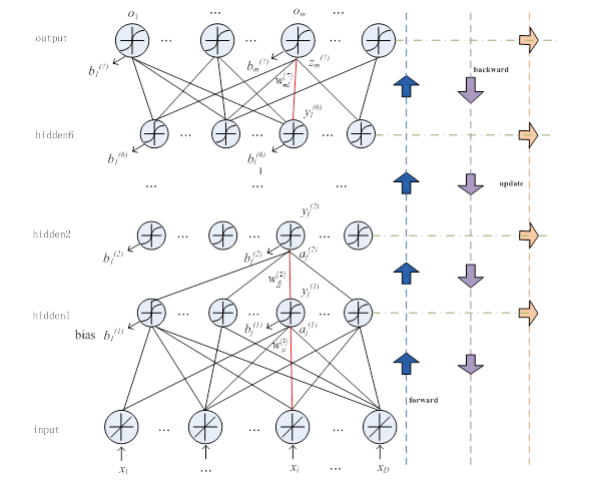
\includegraphics[keepaspectratio=true,width=\dimmin{}{\dimwidth{0.90}}]{images/2016-02-21-21-15-24-}{}\mdline{127}%mdk

%mdk-data-line={130}
\mdhr{}%mdk

%mdk-data-line={131}
\noindent\mdline{131}\mdcaption{\textbf{Figure~\mdcaptionlabel{5}.}~\mdcaptiontext{\mdcode{DNN} structure}}%mdk
%mdk
\end{mdcenter}\label{fig-figure}%mdk
%mdk
\end{figure}%mdk

%mdk-data-line={133}
\subsection{\mdline{133}3.2.\hspace*{0.5em}\mdline{133}Coarse Grain Parallelism}\label{sec-coarse-grain-parallelism}%mdk%mdk

%mdk-data-line={134}
\noindent\mdline{134}To implenment coarse grain parallelism we hope that each thread/process finish large subcomponents. To achieve this goal \mdline{134}\mdcode{DNN}\mdline{134} program should be divided into (mostly) independent and similar proportions, and every proportion should be as large as possible. But considering the structure of \mdline{134}\mdcode{DNN}\mdline{134} the default ordering of \mdline{134}\mdcode{dnn*}\mdline{134} series couldn\mdline{134}'\mdline{134}t be changed, neither does the processing of file-reading. So in our opinion it\mdline{134}'\mdline{134}s difficult to implement coarse grain parallelism without any change to \mdline{134}\mdcode{DNN}\mdline{134} structure and its dataset.%mdk

%mdk-data-line={136}
\section{\mdline{136}4.\hspace*{0.5em}\mdline{136}Performance Optimization Methods}\label{sec-performance-optimization-methods}%mdk%mdk

%mdk-data-line={138}
\subsection{\mdline{138}4.1.\hspace*{0.5em}\mdline{138}Compiler Assisted Offload}\label{sec-compiler-assisted-offload}%mdk%mdk

%mdk-data-line={140}
\subsubsection{\mdline{140}4.1.1.\hspace*{0.5em}\mdline{140}Scope of Offloaded Sections}\label{sec-scope-of-offloaded-sections}%mdk%mdk

%mdk-data-line={141}
\noindent\mdline{141}We have talked about the common structure of \mdline{141}\mdcode{DNN}\mdline{141} series. In their \mdline{141}\mdcode{for}\mdline{141} loop there are serial processing and \mdline{141}\mdcode{MKL}\mdline{141} function appear alternately, and serial processing modifies data which is used as input in next \mdline{141}\mdcode{cblas\_sgemm}\mdline{141}function. Data change between \mdline{141}\mdcode{MIC}\mdline{141} and \mdline{141}\mdcode{CPU}\mdline{141} is slow because of \mdline{141}\mdcode{PCI-E}\mdline{141} speeds so the best known methods\mdline{141}[\mdcite{effective_use}{3}]\mdline{141} is to make the whole section of code an offload unit, which could reduce most of data transfer. In addition, because we nearly make the three \mdline{141}\mdcode{dnn}\mdline{141} functions offload units, data transfer between them is less. SO, all we need do is to transfer input data in the start of \mdline{141}\mdcode{for~loop}\mdline{141} from \mdline{141}\mdcode{CPU}\mdline{141} to \mdline{141}\mdcode{MIC}\mdline{141} and transfer output after loop to \mdline{141}\mdcode{CPU}\mdline{141}. \mdline{141}\mdcode{dnn}\mdline{141} Function is like this (issues about array transfer discussed below):%mdk
\begin{mdpre}%mdk
\noindent~~extern~{\mdcolor{maroon}"}{\mdcolor{maroon}C}{\mdcolor{maroon}"}~{\mdcolor{navy}int}~dnn***({\mdcolor{teal}NodeArg}~\&nodeArg)\\
\{\\
~~~~{\mdcolor{darkgreen}/*}{\mdcolor{darkgreen}~Variables~definition~}{\mdcolor{darkgreen}*/}\\
~~~~{\mdcolor{navy}float}~~*d\_X~=~nodeArg.d\_X;\\
~~~~~~...\\
~~~~\\
~~~~\#pragma~offload~target(mic)\textbackslash{}\\
~~~~in(pd\_Y:length({\mdcolor{purple}0})~{\mdcolor{teal}REUSE})\textbackslash{}\\
~~~~in(pd\_W:length({\mdcolor{purple}0})~{\mdcolor{teal}REUSE})\textbackslash{}\\
~~~~...\\
~~~~\{\\
~~~~~~{\mdcolor{darkgreen}/*}{\mdcolor{darkgreen}~Preprcess~function~func1~}{\mdcolor{darkgreen}*/}\\
~~~~~~func1(...);\\
\\
~~~~~~{\mdcolor{darkgreen}/*}{\mdcolor{darkgreen}~a~for~loop~where~a~function,~a~MKL~\textbackslash{}}\\
{\mdcolor{darkgreen}~~~~~~and~another~function~are~invoked~oderly~}{\mdcolor{darkgreen}*/}\\
\\
~~~~~~{\mdcolor{navy}for}~({\mdcolor{navy}int}~i~=~num;~...)~\{\\
~~~~~~~~~~func2(...);\\
~~~~~~~~~~cblas\_sgemm({\mdcolor{teal}CblasRowMajor},~{\mdcolor{teal}CblasNoTrans},~...);\\
~~~~~~~~~~func3(...);\\
~~~~~~\}\\
~~~~\}~\\
~~~~{\mdcolor{navy}return}~{\mdcolor{purple}0};\\
\}\\
%mdk
\end{mdpre}
%mdk-data-line={171}
\subsubsection{\mdline{171}4.1.2.\hspace*{0.5em}\mdline{171}Dimensionality Reduction}\label{sec-dimensionality-reduction}%mdk%mdk

%mdk-data-line={172}
\noindent\mdline{172}As we know, \mdline{172}\mdcode{MIC}\mdline{172} disallow specifying array of pointer, aka. multi-dimension array, to be use in \mdline{172}\mdcode{in}\mdline{172} or \mdline{172}\mdcode{out}\mdline{172} clauses. To cap it all element in those arrays used in \mdline{172}\mdcode{DNN}\mdline{172} aren\mdline{172}'\mdline{172}t stored consecutively in memory and have different size. So it\mdline{172}'\mdline{172}s necessary for us to calculate array size to allocate one-dimension array. Code like this:%mdk
\begin{mdpre}%mdk
\noindent~~~~{\mdcolor{teal}W\_len}~=~{\mdcolor{purple}0};\\
~~~~{\mdcolor{darkgreen}/*}{\mdcolor{darkgreen}~calculate~element~size~}{\mdcolor{darkgreen}*/}\\
~~~~{\mdcolor{navy}for}~({\mdcolor{navy}int}~i~=~{\mdcolor{purple}1};~i~\textless{}~dnnLayerNum;~i++)~\{\\
~~~~~~~~{\mdcolor{teal}W\_pos}[i~-~{\mdcolor{purple}1}]~=~{\mdcolor{teal}W\_len};\\
~~~~~~~~{\mdcolor{teal}W\_len}~+=~{\mdcolor{darkgreen}/*}{\mdcolor{darkgreen}~i-st~element~size~}{\mdcolor{darkgreen}*/};\\
~~~~\}\\
~~~~{\mdcolor{darkgreen}/*}{\mdcolor{darkgreen}~allocate~memory~}{\mdcolor{darkgreen}*/}\\
~~~~pd\_W~=~({\mdcolor{navy}float}~*)mkl\_malloc({\mdcolor{teal}W\_len}~*~sizeof({\mdcolor{navy}float}),~{\mdcolor{purple}64});\\
~~~~{\mdcolor{darkgreen}/*}{\mdcolor{darkgreen}~build~two-dimension~array~}{\mdcolor{darkgreen}*/}\\
~~~~{\mdcolor{navy}for}~({\mdcolor{navy}int}~i~=~{\mdcolor{purple}0};~i~\textless{}~dnnLayerNum~-~{\mdcolor{purple}1};~i++)~\{\\
~~~~~~~~d\_W[i]~=~pd\_W~+~{\mdcolor{teal}W\_pos}[i];\\
~~~~\}\\
%mdk
\end{mdpre}
%mdk-data-line={189}
\subsection{\mdline{189}4.2.\hspace*{0.5em}\mdline{189}\mdcode{OpenMP}\mdline{189} Optimization}\label{sec-openmp-optimization}%mdk%mdk

%mdk-data-line={190}
\noindent\mdline{190}To maximize the utilization it\mdline{190}'\mdline{190}s better to execute multithreading application in \mdline{190}\mdcode{MIC}\mdline{190}.\mdline{190}[\mdcite{effective_use}{3}]\mdline{190}%mdk

%mdk-data-line={192}
\subsection{\mdline{192}4.3.\hspace*{0.5em}\mdline{192}Alignment}\label{sec-alignment}%mdk%mdk

%mdk-data-line={194}
\subsection{\mdline{194}4.4.\hspace*{0.5em}\mdline{194}Environmental Variables Settings}\label{sec-environmental-variables-settings}%mdk%mdk

%mdk-data-line={195}
\subsubsection{\mdline{195}4.4.1.\hspace*{0.5em}\mdline{195}\mdcode{MKL\_DYNAMIC=true}\mdline{195}:}\label{sec-mkl_dynamictrue-}%mdk%mdk

%mdk-data-line={196}
\noindent\mdline{196}This option may reduce possible oversubscription from MKL threading. It leads to a dynamic reduction of number of OpenMP\mdline{196}*\mdline{196} threads based on analysis of system workload.%mdk

%mdk-data-line={198}
\subsubsection{\mdline{198}4.4.2.\hspace*{0.5em}\mdline{198}\mdcode{MKL\_NUM\_THREADS=50~OMP\_NUM\_THREADS=50}\mdline{198}:}\label{sec-mkl_num_threads50-omp_num_threads50-}%mdk%mdk

%mdk-data-line={199}
\noindent\mdline{199}\mdcode{MKL}\mdline{199} function could decide whether to be threaded after a runtime check.\mdline{199}~[\mdcite{mkl_threads}{1}, \mdcite{paramkl}{4}]\mdline{199} Those variables are maximum threads we allow to create.%mdk

%mdk-data-line={201}
\subsubsection{\mdline{201}4.4.3.\hspace*{0.5em}\mdline{201}\mdcode{MIC\_USE\_2MB\_BUFFERS=100M}}\label{sec-mic_use_2mb_buffers100m}%mdk%mdk

%mdk-data-line={202}
\noindent\mdline{202}2MB pages are also needed. the 2MB pages in compiler-assisted offload are used to improve data transfer performance\mdline{202}[\mdcite{page_file}{5}]\mdline{202}, and they could be enabled using the \mdline{202}\mdcode{MIC\_USE\_2MB\_BUFFERS}\mdline{202} variable.%mdk

%mdk-data-line={204}
\section{\mdline{204}5.\hspace*{0.5em}\mdline{204}Testing Process and Results on the CPU+MIC Platform}\label{sec-testing-process-and-results-on-the-cpumic-platform}%mdk%mdk

%mdk-data-line={207;out/document-bib.bbl.mdk:1}
%mdk-data-line={207;out/document-bib.bbl.mdk:2}
\mdsetrefname{References}%mdk
{\mdbibindent{0}%mdk
\begin{thebibliography}{5}%mdk
\label{sec-bibliography}%mdk

%mdk-data-line={reference.bib:23}
\bibitem{mkl_threads}Konstantin Arturov. \emph{Recommended Settings for Calling Intel MKL Routines from Multi-Threaded Applications}. Intel, https://software.intel.com/en-us/articles/recommended-settings-for-calling-intel-mkl-routines-from-multi-threaded-applications.\label{mkl_threads}%mdk%mdk

%mdk-data-line={reference.bib:1}
\bibitem{mkl-mic}Noah Clemons. \emph{Recommendations to Choose the Right MKL Usage Model for Xeon Phi}. Intel, https://software.intel.com/en-us/articles/recommendations-to-choose-the-right-mkl-usage-model-for-xeon-phi. Mar. 2013.\label{mkl-mic}%mdk%mdk

%mdk-data-line={reference.bib:37}
\bibitem{effective_use}Kevin Davis. \emph{Effective Use of the Intel Compiler’s Offload Features}. Intel, https://software.intel.com/en-us/articles/effective-use-of-the-intel-compilers-offload-features.\label{effective_use}%mdk%mdk

%mdk-data-line={reference.bib:12}
\bibitem{paramkl}\emph{Parallelism in the Intel® Math Kernel Library}. Intel, https://software.intel.com/en-us/articles/parallelism-in-the-intel-math-kernel-library.\label{paramkl}%mdk%mdk

%mdk-data-line={reference.bib:31}
\bibitem{page_file}Zhang Z.~\emph{Performance Tips of Using Intel® MKL on Intel® Xeon Phi™ Coprocessor}. Intel, https://software.intel.com/en-us/articles/performance-tips-of-using-intel-mkl-on-intel-xeon-phi-coprocessor.\label{page_file}%mdk%mdk
\par%mdk
\end{thebibliography}}%mdk%mdk%mdk


\end{document}
